\section{Alternate Protocol 3: Searching the ELM database using REST
API}\label{alternate-protocol-3-searching-the-elm-database-using-rest-api}

Many researchers are interested in large-scale analyses rather than
information about individual protein sequences. To this end, individual
queries to the ELM webserver with a single protein id at a time, are not
practical.

For this reason, as much information as possible is made available via a
REST interface (\cite{Fielding_2002}). This allows the user to interact
with the ELM database and ELM webserver via scriptable URL requests.
Each request can easily be tested in the browser before it is being
automated in a script.

In this section we will explore the various ways in which data can
downloaded both in using the browser as well as via the commandline.

\subsection{Necessary Resources}\label{necessary-resources-3}

\subsubsection{Software}\label{software-1}

Ideally use \texttt{curl} https://curl.haxx.se/ on the commandline. This
program can be launched from the terminal in any of the major operating
systems: OSX, Windows and Linux. Of course \texttt{curl} is only one of
many different ways to access web content programatically, and we
suggest anyone to use which ever program they feel is better suited for
their tasks.

\subsection{Downloading all ELM
classes}\label{downloading-all-elm-classes}

\begin{figure}[htbp]
\centering
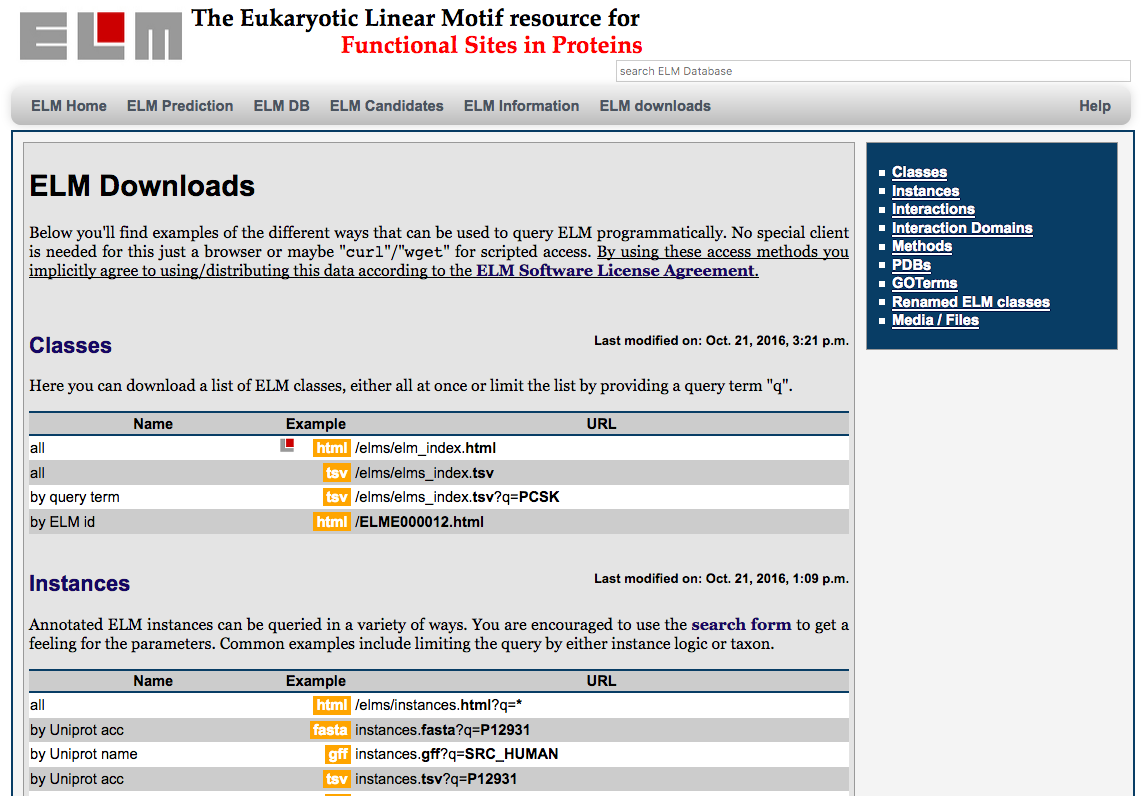
\includegraphics[width=\textwidth]{Figures/BACT_2/elm_downloads_html.png}
\caption{
caption
}
\end{figure}

\textbf{Figure ELM-Downloads:} The ELM downloads page, which holds
information about the different types of data (such as ``Classes'',
``Instances'', etc; see menu to the right) that can be obtained from the
server. The orange boxes are clickable links, the URL following them are
used to highlight the URL scheme used by the server (bold font denotes
specifics used in the examples such as query terms, or formats).

step 1. Direct your browser to the URL `http://elm.eu.org/downloads' or
select `ELM Downloads' from the main Menu (Figure ELM-Downloads) This
webpage contains links and descriptions on how to download ELM data in
text format. The datasets are split into several smaller collections
(for example ``Classes'', ``Instances'', etc). Each table contains links
(in orange) to download the data in various formats.

\sdesc{
Each table also shows the `last modified date' indicating when the data
was last updated. This is useful if you want to know when to update your
local data with the most up to date ELM data.
}

step 2. Click on the first orange `html' link in the table ``Classes''
to navigate to the following URL:
`http://elm.eu.org/elms/elm\_index.html'. This page shows all of the
annotated ELM classes in the database. This page is the same one as
shown in Figure \emph{TP53-BP1-classses}

step 3. Navidate to the folling URL:
`http://elm.eu.org/elms.html?q=CSK', specifying ``q=CSK'' to limit the
list of ELMs to those matching the search query ``CSK''. This page is
again similar to the one shown in Figure \emph{TP53-BP1-classses}, but
with less classes.

\sdesc{
This search result is identical to the result you would obtain by doing
a ``manual'' search on the ELM Classes page
(http://elm.eu.org/elms.html). The column descriptions are also the same
as described in Step XXX in Protocol YYY.
}

\begin{figure}[h!]
\centering
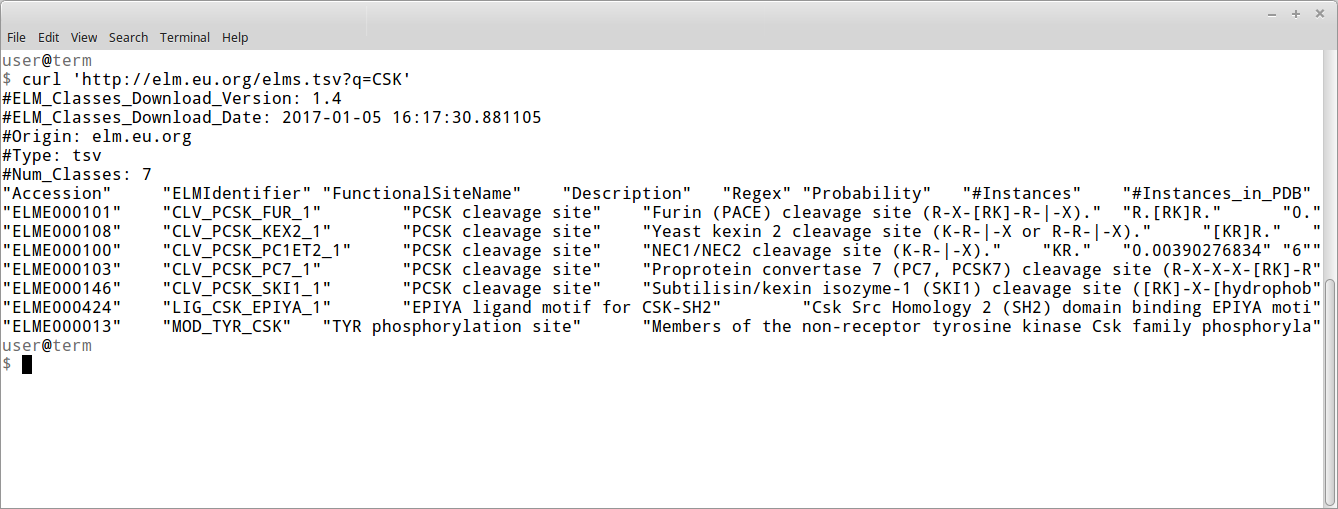
\includegraphics[width=\textwidth]{Figures/BACT_2/elm_curl_classes_CSK.png}
\caption{
\textbf{Figure ELM-Curl-Classes}: Screenshot of a terminal window using
\texttt{curl} to download all ELM classes matching the term `CSK'.
}
\end{figure}

step 4. Open the following URL: `http://elm.eu.org/elms.tsv?q=CSK' to
download a list of classes that match the search query ``CSK'' (as in
the previous step) in the ``tab separated values'' format. By exchanging
the `.html' part of the url with `.tsv', we ask the webserver to give us
the data in TSV (tab-separated values) format.

\sdesc{
Depending on which browser you are using, the file may open directly in
your browser, or you may be prompted to download the file or save it to
a separate location. In the latter two cases you can open the downloaded
file using a (plain) text file viewer, or possible a spreadsheet viewer
(such as Microsoft Excel).
}

step 5. Type the follwing command into a command line terminal to
download the same data from the previous step directly into the
terminal: \texttt{curl 'http://elm.eu.org/elms/elms\_index.tsv?q=CSK'}.
The output should look similar to \emph{Figure ELM-Curl-Classes}. The
column names are still the same ones as shown in the \emph{classes}
table in Figure \emph{BACT-AP2-Elm-classes-downloads}.

\sdesc{
Use the curl option \texttt{-o} to save the results directly to a file.
For example:
\texttt{curl -o classes.tsv 'http://elm.eu.org/elms/elms\_index.tsv?q=CSK'}
will save the data to a file called \emph{classes.tsv}.
}

step 6: To download a list of all motif instances detected in Human P53,
type the followin command into a terminal:
\texttt{curl 'http://elm.eu.org/instances.gff?q=p53\_human'}. The output
should look similar to that shown in figure \emph{Figure ELM-Curl-P53}.
The output is in the ``General Feature Format''
(http://www.ensembl.org/info/website/upload/gff.html\#moreinfo), with
the FASTA formatted sequence appended to the end of the output.

\sdesc{
Many other file formats are available for downloading instances
annotations, including the FASTA, GFF, PIR, or PSI-MI format (either XML
or MiTab) {[}24067240{]}.
}

\begin{figure}[h!]
\centering
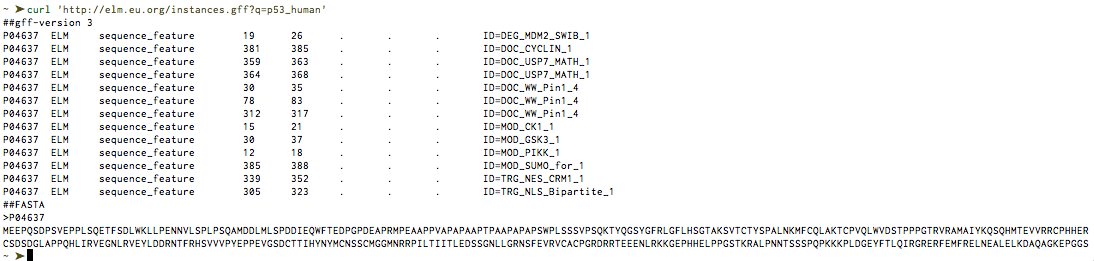
\includegraphics[width=\textwidth]{Figures/BACT_2/elm_curl_instances_p53_human.png}
\caption{
\textbf{Figure ELM-Curl-Instances-P53}: Screenshot of a terminal window
using \texttt{curl} to download all ELM instances annotated for sequence
p53\_human.
}
\end{figure}

step 7. To download a list of all instances matchin th search query
``CLV'' in the yellow fever mosquito (Aedes agypti), enter the following
command into a terminal: `curl
`http://elm.eu.org/instances.tsv?q=CLV\&taxon=aedes+aegypti'. In general
any species name can be used, always replacing the ``space'' with a
``+''. This should return a single instance, the only one matching CLV
in A. aegypti.

step 8. More data (interactions, domains, methods, etc.) can be
downloaded from ELM in analogous fashion as shown in the preceeding
steps. Take a look at the ELM Downloads page
(http://elm.eu.org/downloads, Figure \emph{BACT-AP2-Elm-downloads}) for
an overview of which datasets can be downloaded, and what the different
possible filters and formats are for each dataset.

\% NOTE: TODO: Mention ELM software license agreement?

\section{Guidelines for Interpreting
Results}\label{guidelines-for-interpreting-results}

\emph{instructions: A brief discussion of the theory and applications of
your}

\emph{notes: Maybe mention how findings are relevant to the lab? For
example: Manually annotated content should be reliable, although one
should look at the `confidence' in the instance annotation. Predictions
are probably trustworthy, but you need to take into account the
`confidence score', and other features like whether its in a domain,
etc\ldots{}}

\section{Commentary:}\label{commentary}

\emph{instructions: A brief discussion of the theory and applications of
your}

\subsection{Background Information}\label{background-information}

\textbf{Im still not sure what's going to happen here}

In order to interpret the data contained in ELM and the results produced
by the ELM prediction tool, it is important to have a basic
understanding of SLiM's and how they are affected by their structural
and biological context.

Taking into account additional information, besides a match to a
sequence pattern defining a SLiM, can greatly narrow the selection of
putative motifs for experimental validation.

SLiM's operate via with interactions with other proteins, typically the
surface of a globular, domain in a protein, although some are known to
bind to disordered regions. As their name suggests, SLiMs are compact,
being composed of a limited number of adjacent amino acids. Most of a
motif's binding specificity however is conferred by only a subset of
these amino acids. Those few residues that directly interact with the
binding partner are evolutionary conserved, although in many cases a
subset of amino acids that share certain properties (such as similar
charge, size or hydrophobicity) are allowed in these hotspot positions.
In the motif positions that contribute little to the interaction, there
are even less constraints, i.e.~a broader range of amino acids is
allowed in these positions (\cite{21909575}). A first consequence of
this degeneracy is that SLiMs co-operatively engage in interactions of
relatively low affinity. Hence these binding events are transient and
reversible, and can be readily modulated, for instance by PTM.

\begin{figure}[h!]
\centering
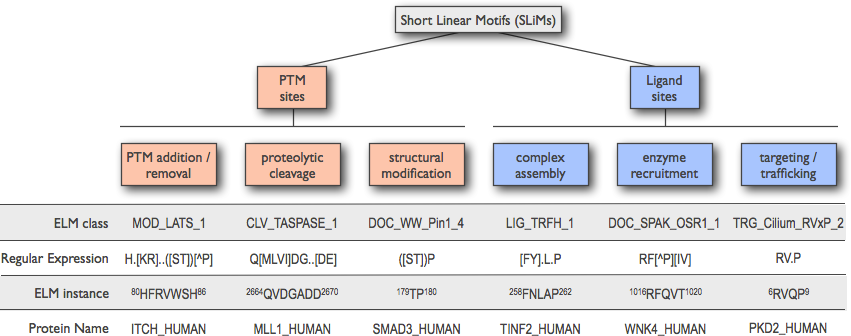
\includegraphics[width=\textwidth]{Figures/functional_classification_of_SLiMs.png}
\caption{
\textbf{Figure functional\_classification\_of\_SLiMs} For each ELM
class, the functional category to which it belongs is indicated by a
three-letter prefix. Each ELM class is defined by a regular expression.
Peptide sequences in proteins that match the regular expression of a
specific ELM class and that were experimentally validated to be
functional motifs are captured as ELM instances of that class. Degrons
are a specific subtype of enzyme-recruiting docking motifs (see text for
a detailed description).
}
\end{figure}

\subsection{Critical Parameters and
Troubleshooting}\label{critical-parameters-and-troubleshooting}

\emph{instructions: optionally 2 separate sections.}

\section{Internet Resources with
Annotations}\label{internet-resources-with-annotations}

http://www.clustal.org/omega Clustal Omega (\cite{21988835}) is a tool
for the alignment of multiple nucleic acid and protein sequences.

http://www.jalview.org Jalview (\cite{19151095}) is a Java desktop
application (and browser applet) that employs web services for sequence
alignment and visualization.

http://proviz.ucd.ie ProViz (\cite{27085803}) is an interactive protein
exploration tool, which searches several databases for information about
a given query protein. Data relevant to the protein like an alignment of
homologues, linear motifs, post translational modifications, domains,
secondary structure, sequence variations and others are graphically
represented relative to their position in the protein.
